\begin{figure}[t]
  \usetikzlibrary{shapes.arrows, fadings}
  \definecolor{LightColor}{rgb}{1.0,0.901,0.805}

  \definecolor{tile0}{HTML}{DABDE4}
  \definecolor{tile1}{HTML}{B8DBF4}
  \definecolor{tile2}{HTML}{B5EDCD}
  \definecolor{tile3}{HTML}{FBEBA7}
  \definecolor{tile4}{HTML}{F9C1BB}
  \definecolor{tile5}{rgb}{1, 1, 1}

  \tikzstyle{array_element}=[rectangle,
                             minimum height=1cm, 
                             minimum width=1cm, 
                             minimum size=1cm,
                             draw=black,
                             rounded corners=2.5 ]
  \tikzstyle{grid_element}=[rectangle,
                            minimum height=1.5cm, 
                            minimum width=1.5cm, 
                            draw=black,
                            rounded corners=2.5 ]
  \tikzstyle{grid_element_big}=[rectangle, 
                               minimum height=2cm, 
                               minimum width=2cm, 
                               draw=black,
                               rounded corners=2.5 ]
 \tikzstyle{grid_element_bigly}=[rectangle, 
                               minimum height=3cm, 
                               minimum width=3cm, 
                               draw=black,
                               rounded corners=2.5 ]


\begin{adjustbox}{minipage=\textwidth, scale=0.5}
  \centering
  \begin{tikzpicture}
    \node at (-4.cm, 4cm) (light_list_name) [anchor=west] {Global Light List:};
    \node at (-4.cm, 2cm) (light_list_name) [anchor=west] {Light Index List:};
    \node at (-4.cm, -1.5cm) (light_list_name) [anchor=west] {Octree:};
    \node at (2.75cm, -1.5cm) (light_list_name) [anchor=west] {Spatial Hash Functions:};
    

    \foreach \l in {0,...,6} {
      \node at (1cm * \l + 1cm, 4cm) (light_\l) [array_element,fill={LightColor}] {$\mathbf{l}_\l$};
    }
    \node at (1cm * 7, 4cm) [array_element, fill={LightColor}, ] {};
    \node at (1cm * 7.325, 4cm) [rectangle,
                                 minimum height=1.2cm,
                                 minimum width=0.6cm,
                                 fill={white},
                                 draw=white] {};
    \node at (1cm * 7, 4cm) [rectangle,                    
                             minimum height=0.98cm, 
                             minimum width=0.2cm, 
                             shading = axis,
                             shading angle=90,
                             left color=LightColor ] {};
                             
    \node at (1cm * 7, 4cm) [rectangle, minimum height=1cm, minimum width=1cm] {$\dots$};

    \node at (1cm * 0, 2cm) [array_element,
                              fill={white}, ] {};
    \node at (1cm * -0.325, 2cm) [rectangle,
                                  minimum height=1.2cm,
                                  minimum width=0.6cm,
                                  fill={white},
                                  draw=white] {};
    \node at (1cm * 0, 2cm) [rectangle,
                              minimum height=1cm,
                              minimum width=1cm] {$\dots$};


    \foreach \i/\l in {0/0} {
      \node at (1cm * \i +1cm, 2cm) (light_index_\i) [array_element, fill={tile0}] {\l};
      \draw[-latex] (light_index_\i.north) -- (light_\l.south);
    }
    \foreach \i/\l in {1/0, 2/1, 3/4} {
      \node at (1cm * \i  +1cm, 2cm) (light_index_\i) [array_element, fill={tile1}] {\l};
      \draw[-latex] (light_index_\i.north) -- (light_\l.south);
    }
    \foreach \i/\l in {4/2, 5/4} {
      \node at (1cm * \i  +1cm, 2cm) (light_index_\i) [array_element, fill={tile2}] {\l};
      \draw[-latex] (light_index_\i.north) -- (light_\l.south);
    }
    \foreach \i/\l in {6/5} {
      \node at (1cm * \i  +1cm, 2cm) (light_index_\i) [array_element, fill={tile3}] {\l};
      \draw[-latex] (light_index_\i.north) -- (light_\l.south);
    }
    \foreach \i/\l in {7/3, 8/5, 9/6} {
      \node at (1cm * \i  +1cm, 2cm) (light_index_\i) [array_element, fill={tile4}] {\l};
      \draw[-latex] (light_index_\i.north) -- (light_\l.south);
    }
    \node at (1cm * 10  +1cm, 2cm) [array_element,
                              fill={white}, ] {};
    \node at (1cm * 10.325  +1cm, 2cm) [rectangle,
                                  minimum height=1.2cm,
                                  minimum width=0.6cm,
                                  fill={white},
                                  draw=white] {};
    \node at (1cm * 10  +1cm, 2cm) [rectangle,
                              minimum height=1cm,
                              minimum width=1cm] {$\dots$};

\node[inner sep=0pt] (level_0) at (-1.25cm,-5.5cm - 1cm)
    {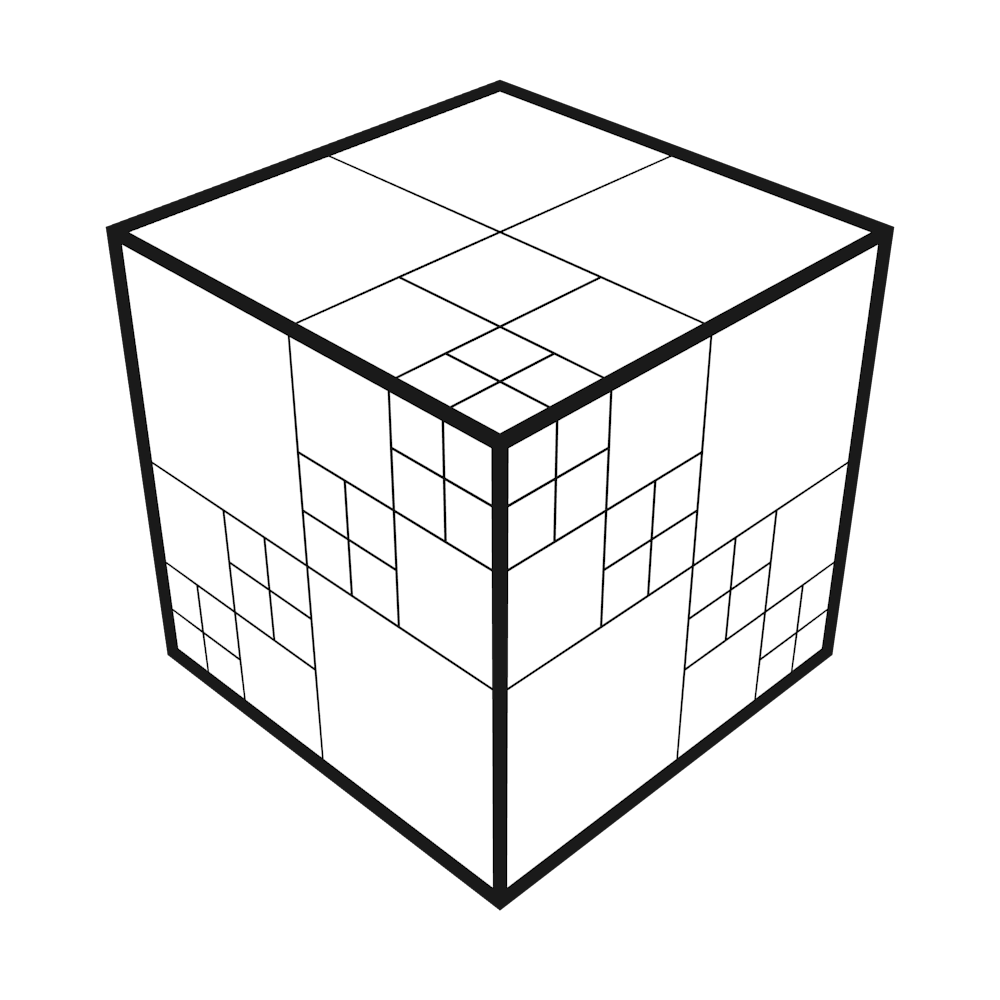
\includegraphics[width=6.5cm]{./img/raw/hs-datastructuren-overzicht/octree.png}};
    
\node at (4cm, -2.cm) {$\vdots$};
\node at (4cm, -10.5cm) {$\vdots$};




\node[inner sep=0pt] (level_0) at (4.0cm,-3cm  - 1.5cm)
    {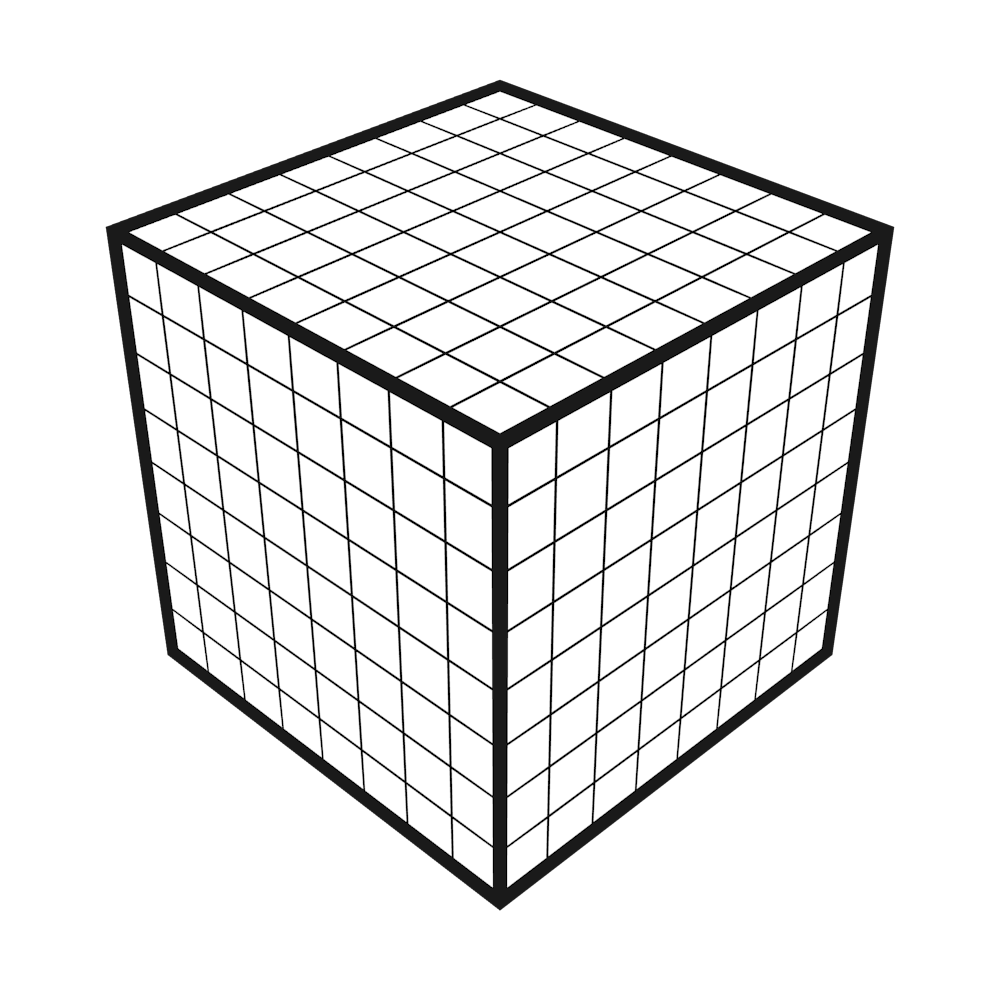
\includegraphics[width=3cm]{./img/raw/hs-datastructuren-overzicht/img1.png}};
\node[inner sep=0pt] (level_0) at (6.25cm,-2.75cm  - 1.5cm)
    {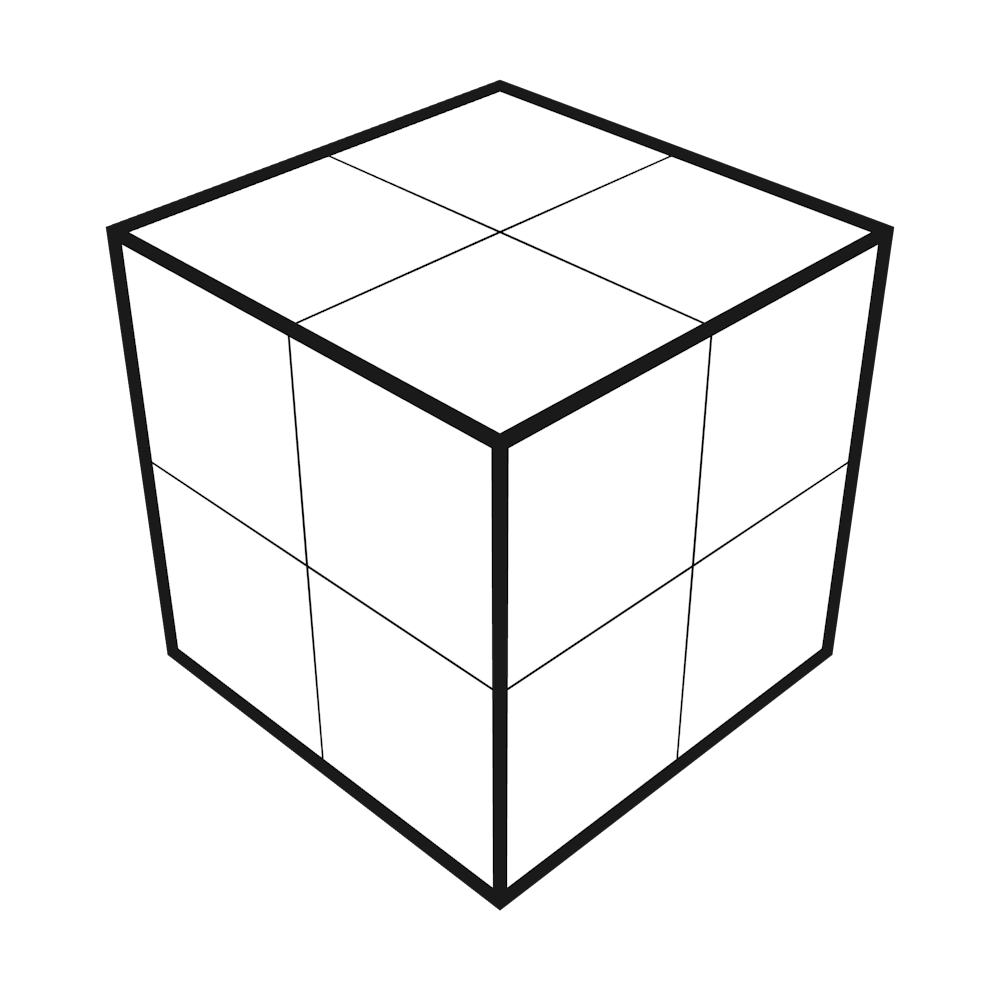
\includegraphics[width=2cm]{./img/raw/hs-datastructuren-overzicht/img2.png}};
\node[inner sep=0pt] (level_0) at (8.5cm,-3cm  - 1.5cm)
    {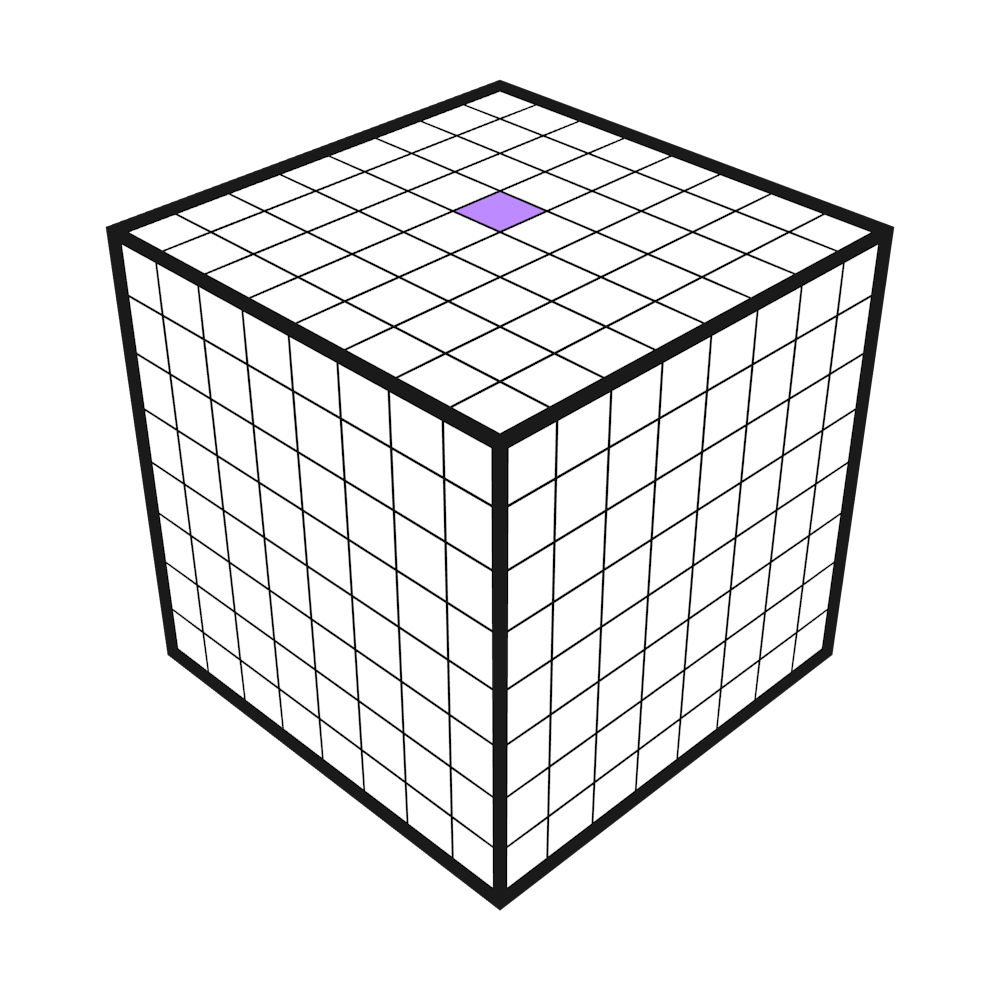
\includegraphics[width=3cm]{./img/raw/hs-datastructuren-overzicht/img3.png}};
\node[inner sep=0pt] (level_0) at (10.75cm,-2.75cm  - 1.5cm)
    {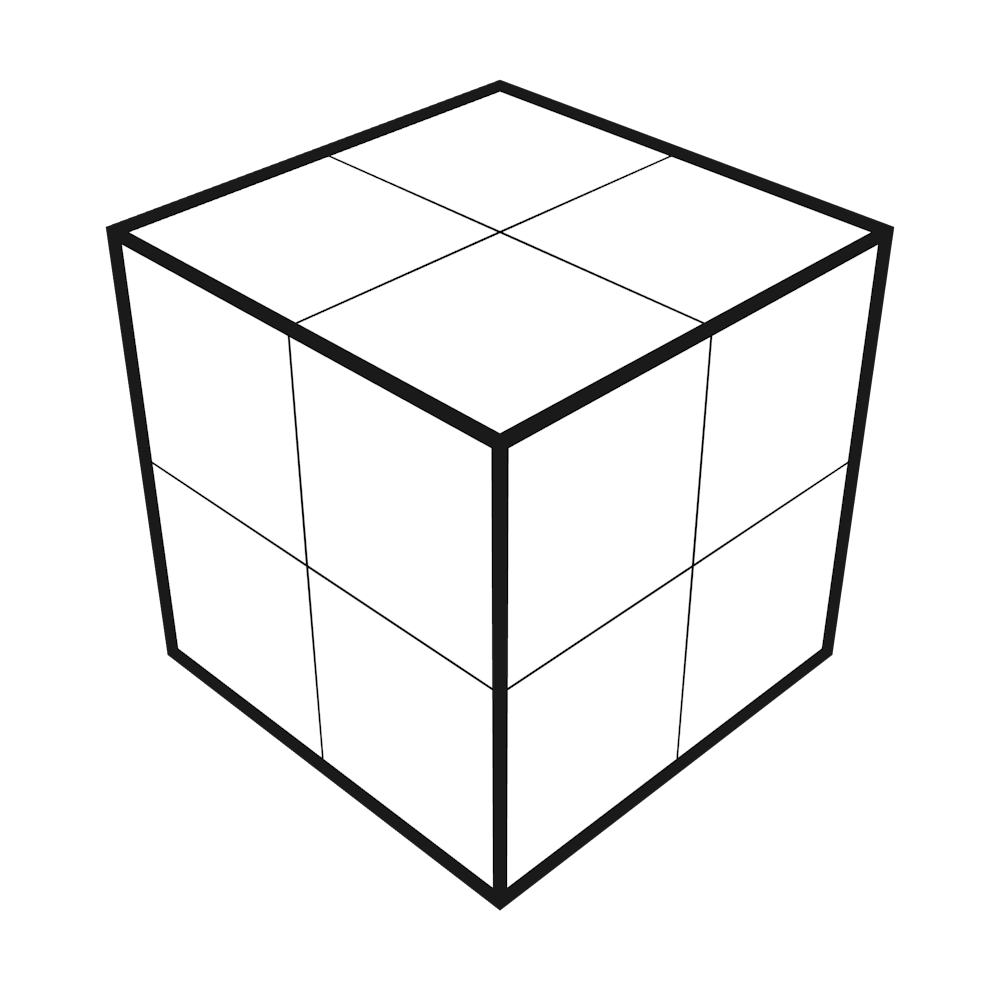
\includegraphics[width=2cm]{./img/raw/hs-datastructuren-overzicht/img2.png}};

\node[inner sep=0pt] (level_0) at (4.0cm,-3cm - 3.75cm  - 1.5cm)
    {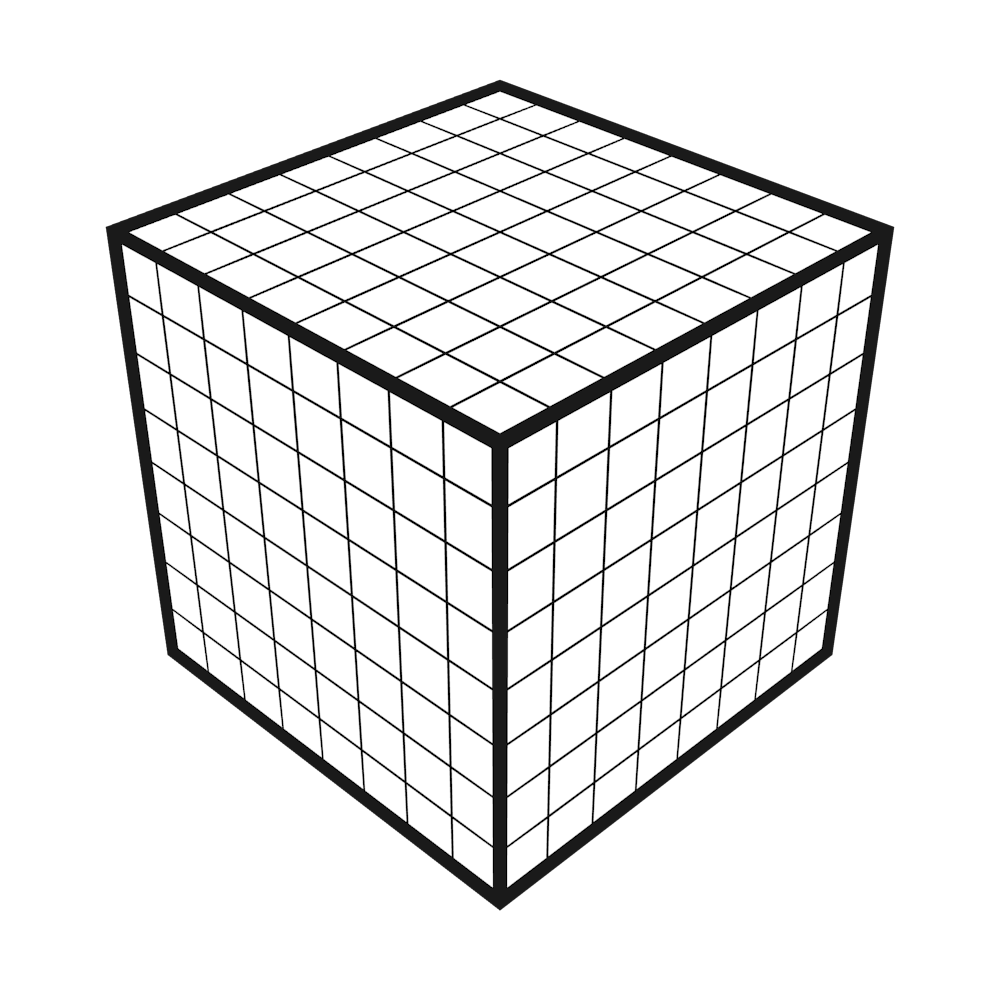
\includegraphics[width=3cm]{./img/raw/hs-datastructuren-overzicht/img1.png}};
\node[inner sep=0pt] (level_0) at (6.25cm,-2.75cm - 3.75cm  - 1.5cm)
    {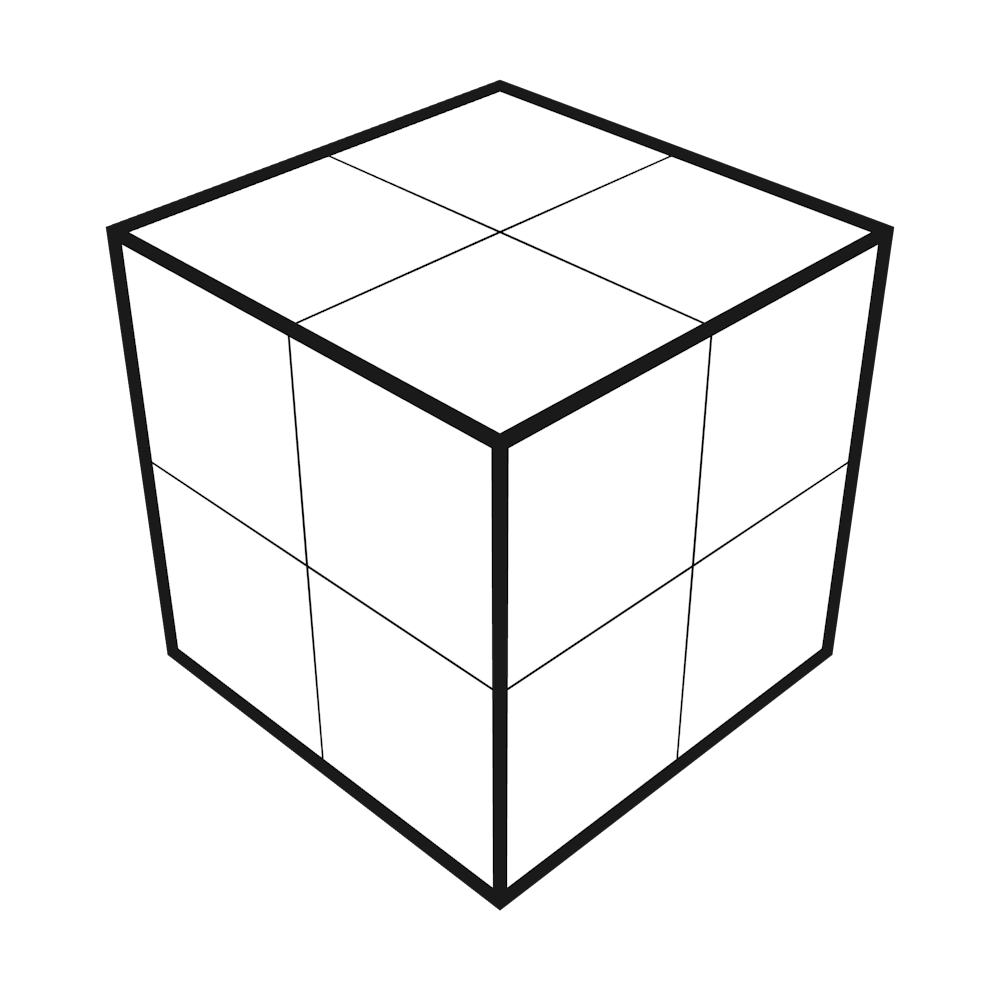
\includegraphics[width=2cm]{./img/raw/hs-datastructuren-overzicht/img2.png}};
\node[inner sep=0pt] (level_0) at (8.5cm,-3cm - 3.75cm  - 1.5cm)
    {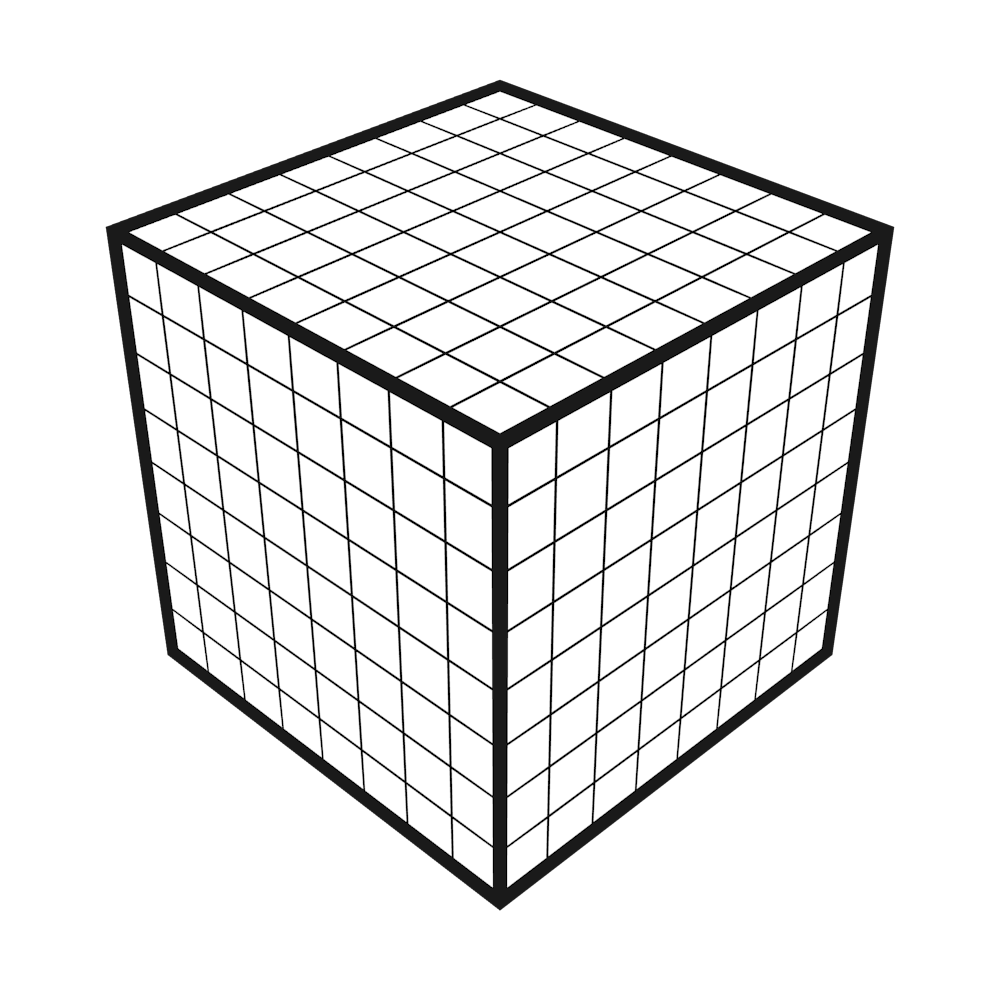
\includegraphics[width=3cm]{./img/raw/hs-datastructuren-overzicht/img1.png}};
\node[inner sep=0pt] (level_0) at (10.75cm,-2.75cm - 3.75cm  - 1.5cm)
    {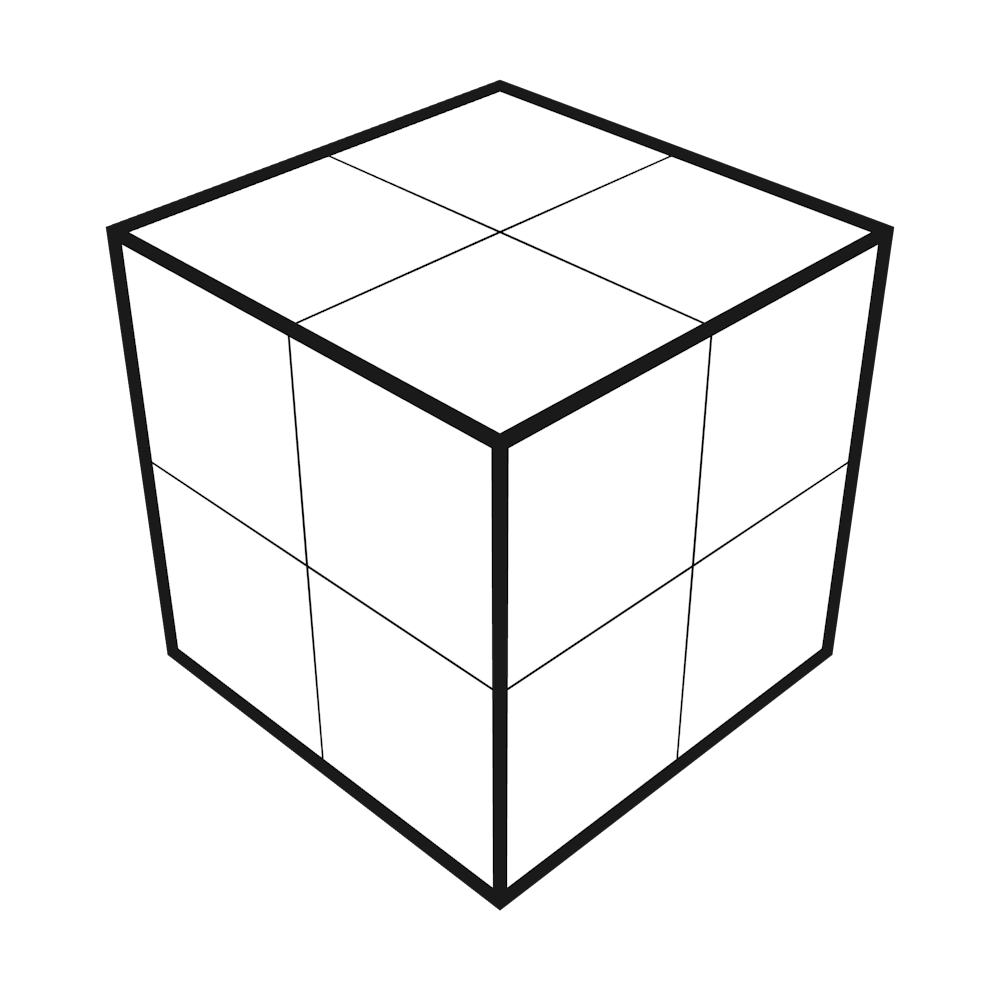
\includegraphics[width=2cm]{./img/raw/hs-datastructuren-overzicht/img2.png}};

\node at (11.75cm, -2.8cm) {\scriptsize layer $i$};
\node at (11.75cm, -2.8cm - 3.75cm) {\scriptsize layer $i + 1$};

\node at (3.0cm, -3.25cm) {$H_{1,i}$};
\node at (5.75cm, -3.25cm) {$\Phi_{1,i}$};
\node at (7.5cm, -3.25cm) {$H_{2,i}$};
\node at (10.25cm, -3.25cm) {$\Phi_{2,i}$};

\node at (3.0cm, -3.25cm -3.75cm) {$H_{1,i + 1}$};
\node at (5.75cm, -3.25cm  -3.75cm) {$\Phi_{1,i + 1}$};
\node at (7.5cm, -3.25cm -3.75cm) {$H_{2,i + 1}$};
\node at (10.25cm, -3.25cm -3.75cm) {$\Phi_{2,i + 1}$};

\node at (2cm, -2.5cm) (l1) {};
\node at (12.75cm, -2.5cm) (l2) {};
\draw[-, gray, very thin] (l1) -- (l2);

\node at (2cm, -2.5cm  -3.75cm) (l1) {};
\node at (12.75cm, -2.5cm  -3.75cm) (l2) {};
\draw[-, gray, very thin] (l1) -- (l2);

\node at (2cm, -2.5cm  -3.75cm -3.75cm) (l1) {};
\node at (12.75cm, -2.5cm  -3.75cm -3.75cm) (l2) {};
\draw[-, gray, very thin] (l1) -- (l2);

\node at (8.35cm, -3.63cm) (l1) {};
\node at (8.625cm, -3.63cm) (l2) {};

    \node at (-2.25cm + 10.75cm, -2cm + 1.5cm) (node_big) [grid_element_big, fill=tile0] {};
    \node at (-3.25cm + 10.75cm , -2cm + 1.5cm) (grid_l) [] {};
    \node at (-1.25cm + 10.75cm, -2cm + 1.5cm) (grid_r) [] {};
    \draw (grid_l.center) -- (grid_r.center);
    \node at (-2.25cm + 10.75cm, -1.5cm + 1.5cm) [] { offset: $\mathit{k}$ };
    \node at (-2.25cm + 10.75cm, -2.5cm + 1.5cm) [] { size: $\mathit{1}$ };

    \node at (-3.25cm + 10.75cm, -3cm + 1.55cm) (node_big_1) {};
    \node at (-1.25cm + 10.75cm, -3cm + 1.55cm) (node_big_2) {};


    \draw[gray] (node_big_1.center) -- (l1.center);
    \draw[gray] (node_big_2.center) -- (l2.center);
    
    \draw[-latex] (node_big.west) -- (light_index_0.south);


  \end{tikzpicture}
  \end{adjustbox}

  \caption{Overview of the data structures of Hashed Shading.}
  \label{fig:hs-data-structures}
\end{figure}
